%------------------------------------------
%	$Id$
%
%	The GMT Documentation Project
%	Copyright (c) 2000-2012.
%	P. Wessel, W. H. F. Smith, R. Scharroo, and J. Luis
%------------------------------------------
%
\chapter{Color Space: The final frontier}
\label{app:I}
\thispagestyle{headings}

\index{Color|(}
\index{Color!HSV system|(}
\index{Color!RGB system|(}

In this Appendix, we are going to try to explain the relationship
between the RGB, CMYK, and HSV color systems so as to (hopefully) make
them more intuitive.  \GMT\ allows users to specify colors in CPT
files in either of these three systems. Interpolation between colors is performed in either RGB or HSV, depending on the specification in the CPT file. Below, we will explain why this all matters.

\section{RGB color system}
Remember your (parents') first color television set? Likely it had three little bright colored squares on it: red, green, and blue. And that is exactly what each color on the tube is made of: varying levels of red, green and blue light. Switch all of them off, $r=g=b=0$, then you have black. All of them at maximum, $r=g=b=255$, creates white. Your computer screen works the same way.

A mix of levels of red, green, and blue creates basically any color imaginable. In \GMT\ each color can be represented by the triplet $r$/$g$/$b$. For example, 127/255/0 (half red, full green, and no blue) creates a color called chartreuse. The color sliders in the graphics program \progname{GIMP} are an excellent way to experiment with colors, since they show you in advance how moving one of the color sliders will change the color. As Figure~\ref{fig:gimp}\emph{a} shows: increase the red and you will get a more yellow color, while lowering the blue level will turn it into brown.

\begin{figure}[b]
   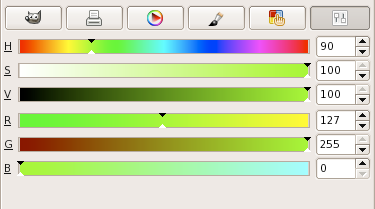
\includegraphics[width=0.47\textwidth,bb=0 0 375 209]{gimp-sliders.png}~\emph{a}\hfill
   \emph{b}~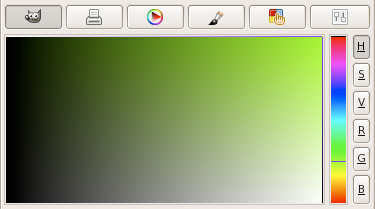
\includegraphics[width=0.47\textwidth,bb=0 0 375 209]{gimp-panel.png}
   \caption{Chartreuse in \protect\progname{GIMP}. (\emph{a}) Sliders indicate how the color is altered when changing the H, S, V, R, G, or B levels. (\emph{b}) For a constant hue (here 90\DS) value increases to the right and saturation increases up, so the ``pure'' color is on the top right.}
   \label{fig:gimp}
\end{figure}

Is chocolate your favorite color, but you do not know the RGB equivalent values? Then look them up in Figure~\ref{fig:RGBchart} or type \progname{man gmtcolors} for a full list. It's 210/105/30. But \GMT\ makes it easy on you: you can specify pen, fill, and palette colors by any of the more than 500 unique colors found in that file.

Are you very web-savvy and work best with hexadecimal color codes as they are used in HTML? Even that is allowed in \GMT. Just start with a hash mark (\texttt{\#}) and follow with the 2 hexadecimal characters for red, green, and blue. For example, you can use \texttt{\#79ff00} for chartreuse, \texttt{\#D2691E} for chocolate.

\begin{figure}
   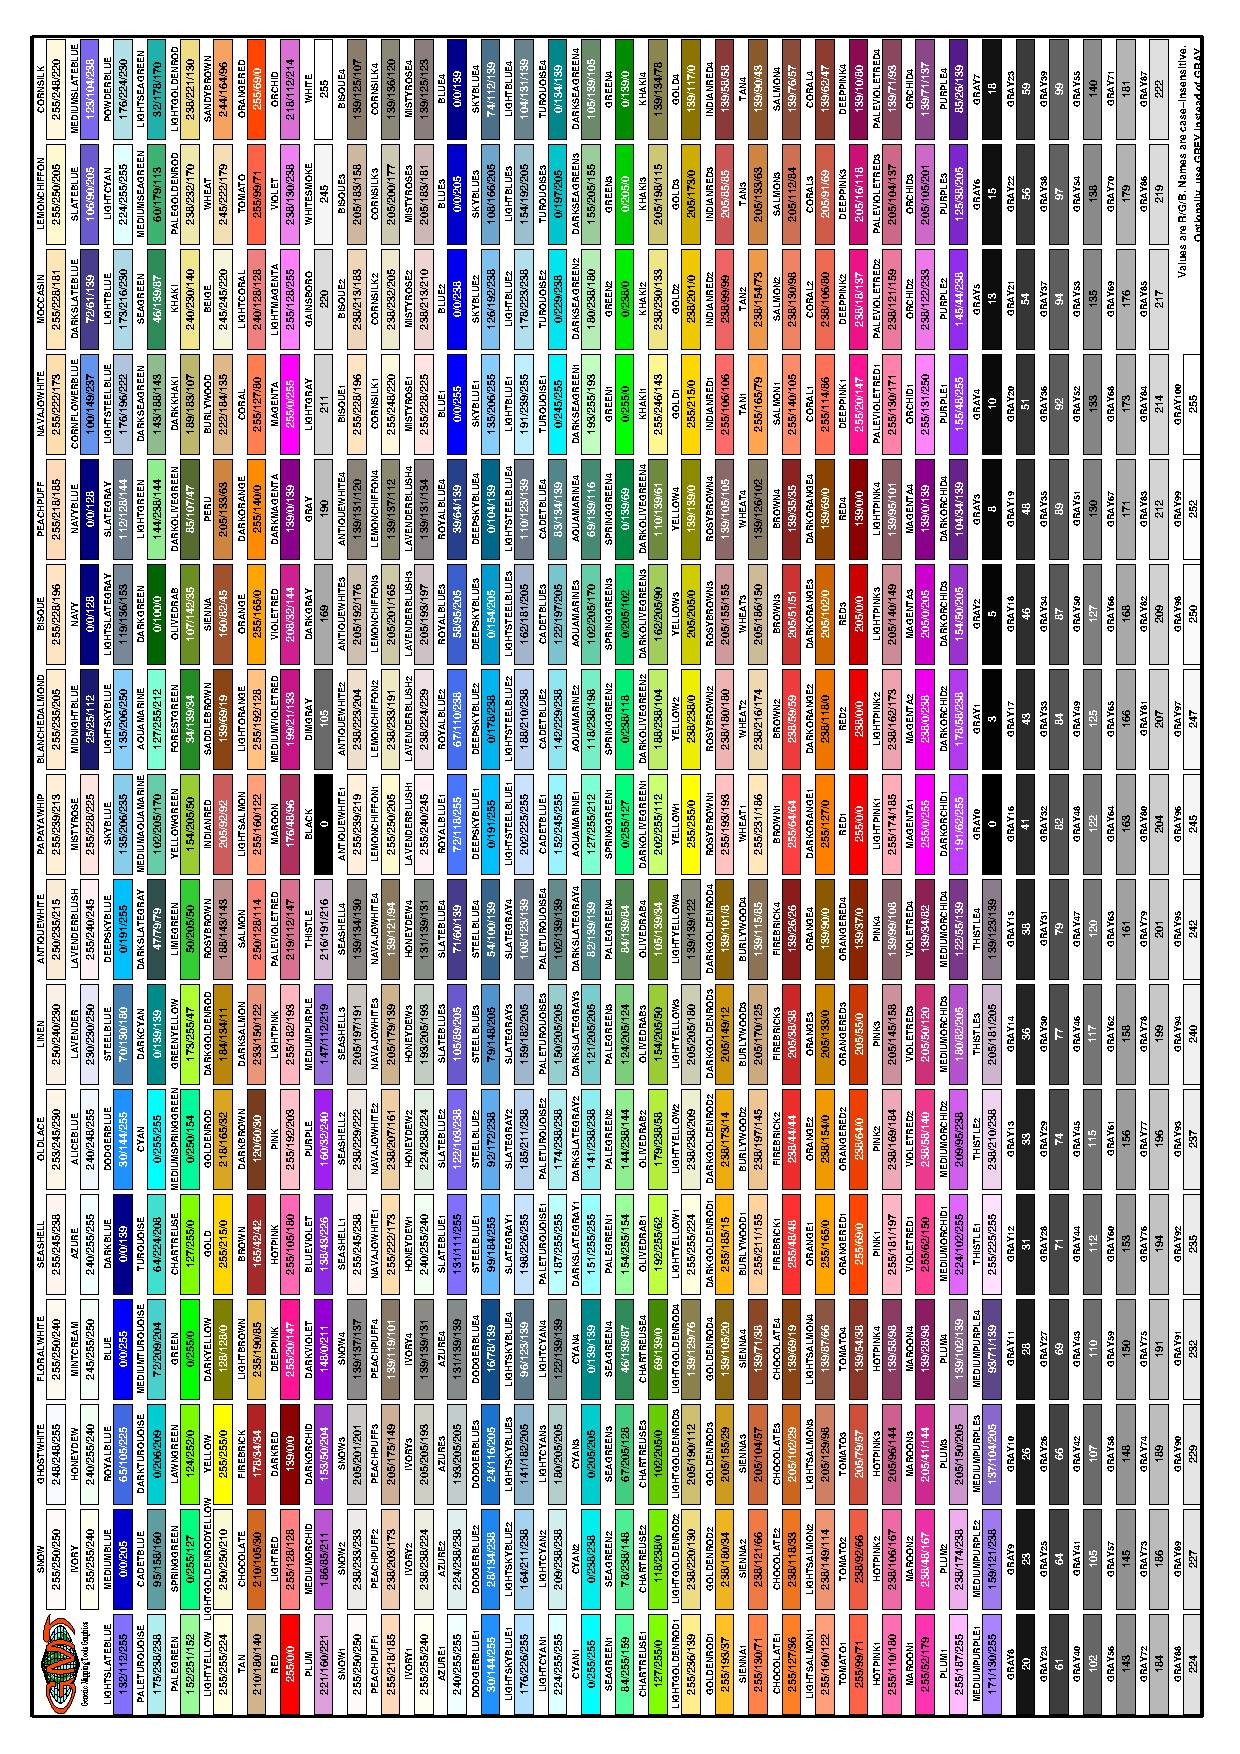
\includegraphics[angle=90,width=\textwidth]{GMT_RGBchart_a4}
   \caption{The 555 unique color names that can be used in GMT. Lower, upper, or mixed cases, as well as the british
   spelling of ``grey'' are allowed. A4, Letter, and Tabloid sized versions of this RGB chart can be found in the
   GMT documentation directory.}
   \label{fig:RGBchart}
\end{figure}

\section{HSV color system}
If you have played around with RGB color sliders, you will have noticed that it is not intuitive to make a chosen color lighter or darker, more saturated or more gray. It would involve changing three sliders. To make it easier to manipulate colors in terms of lightness and saturation, another coordinate system was invented: HSV (hue, saturation, value). Those terms can be made clear best by looking at the color sliders in Figure~\ref{fig:gimp}\emph{a}. Hue (running from 0\DS\ to 360\DS) gives you the full spectrum of saturated colors. Saturation (from 0 to 1, or 100\%) tells you how `full' your color is: reduce it to zero and you only have gray scales. Value (from 0 to 1, or 100\%) will bring you from black to a fully saturated color. Note that ``value'' is not the same as ``intensity'', or ``lightness'', used in other color geometries. ``Brilliance'' may be the best alternative word to describe ``value''. Apple calls it as ``brightness'', and hence refers to HSB for this color space.

Want more chartreuse or chocolate? You can specify them in \GMT\ as 90-1-1 and 25-0.86-0.82, respectively.

\section{The color cube}
We are going to try to give you a geometric picture of color
mixing in RGB and HSV by means of a tour of the RGB cube depicted in Figure~\ref{fig:GMT_example_11}.  The geometric
picture is most helpful, we think, since HSV are not orthogonal
coordinates and not found from RGB by a simple algebraic transformation.
So here goes: Look at the
cube face with black, red, magenta, and blue corners.
This is the $g$ = 0 face.  Orient the cube so that you are
looking at this face with black in the lower left corner.  Now
imagine a right-handed cartesian ($r$,$g$,$b$) coordinate system
with origin at the black point; you are looking at the $g = 0$
plane with $r$ increasing to your right, $g$ increasing
away from you, and $b$ increasing up.  Keep this sense of
($r$,$g$,$b$) as you look at the cube.

Now tip the cube such that the black corner faces down and the white corner up. When looking from the top, you can see the hue, contoured in gray solid lines, running around in 360\DS\ counter-clockwise. It starts with shades of red (0\DS), then goes through green (120\DS) and blue (240\DS), back to red.

On the three faces that are now on the lower side (with the white print) one of ($r$,$g$,$b$) is equal to 0. These three faces meet at the black corner, where $r = g = b = 0$. On these three faces the colors are fully saturated: $s$ = 1. The dashed white lines indicate different levels of $v$, ranging from 0 to 1 with contours every 0.1.

On the upper three faces (with the black print), one of ($r$,$g$,$b$) is equal to the
maximum value.  These three faces meet at the white corner, where
$r = g = b = 255$.  On these three faces value is at
its maximum: $v$ = 1 (or 100\%). The dashed black lines indicate varying levels of saturation: $s$ ranges from 0 to
1 with contours every 0.1.

Now turn the cube around on its vertical axis (running from the black to the white corner). Along the six edges that zigzag around the ``equator'', both saturation and value are maximum, so $s = v = 1$. Twirling the cube around and tracing the zigzag, you will visit six of the eight corners of the
cube, with changing hue ($h$):  red (0\DS), yellow (60\DS), green
(120\DS), cyan (180\DS), blue (240\DS), and magenta
(300\DS). Three of these are the RGB colors; the other three
are the CMY colors which are the complement of RGB and are used in many
color hardcopy devices (see below).  The only cube
corners you did not visit on this path are the black and white corners.
They lie on the vertical axis where hue is undefined and $r = g = b$. Any point on this axis is a shade of gray.

Let us call the points where $s = v = 1$ (points along the RYGCBM path described above) the ``pure'' colors.  If we start at a pure color
and we want to whiten it, we can keep $h$ constant and $v = 1$
while decreasing $s$; this will move us along one of the cube
faces toward the white point.  If we start at a pure color and we want
to blacken it, we can keep $h$ constant and $s = 1$ while decreasing
$v$; this will move us along one of the cube faces toward the black
point.  Any point in ($r$,$g$,$b$) space which can be thought of as a
mixture of pure color + white, or pure color + black, is on a face of
the cube.

The points in the interior of the cube are a little harder to describe.
The definition for $h$ above works at all points in (non-gray)
($r$,$g$,$b$) space, but so far we have only looked at ($s$,
$v$) on the cube faces, not inside it.  At interior points, none
of ($r$,$g$,$b$) is equal to either 0 or 255.  Choose such a point,
not on the gray axis.  Now draw a line through your point so that the
line intersects the gray axis and also intersects the RYGCBM path of
edges somewhere.  It is always possible to construct this line, and
all points on this line have the same hue.  This construction shows
that any point in RGB space can be thought of as a mixture of a pure
color plus a shade of gray.  If we move along this line away from the
gray axis toward the pure color, we are ``purifying'' the color by
``removing gray''; this move increases the color's saturation.  When
we get to the point where we cannot remove any more gray, at least one
of ($r$,$g$,$b$) will have become zero and the color is now fully
saturated; $s = 1$.  Conversely, any point on the gray axis is
completely undersaturated, so that $s = 0$ there.  Now we see that
the black point is special, $s$ is both 0 and 1 at the same time. In other words, at the black point saturation in undefined (and so is hue). The convention is to use $h = s = v = 0$ at this point.

It remains to define value. To do so, try this:
Take your point in RGB space and construct a line through it so that
this line goes through the black point; produce this line from black
past your point until it hits a face on which $v = 1$.  All points
on this line have the same hue.  Note that this line and the line we
made in the previous paragraph are both contained in the plane whose
hue is constant.  These two lines meet at some arbitrary
angle which varies depending on which point you chose.  Thus HSV is
not an orthogonal coordinate system.  If the line you made in the
previous paragraph happened to touch the gray axis at the black point,
then these two lines are the same line, which is why the black point
is special.  Now, the line we made in this paragraph illustrates the
following:  If your chosen point is not already at the end of the
line, where $v = 1$, then it is possible to move along the line in
that direction so as to increase ($r$,$g$,$b$) while keeping the
same hue.  The effect this has on a color monitor is to make the
color more ``brilliant'', your hue will become ``stronger''; if you are already on a plane where
at least one of ($r$,$g$,$b$) = 255, then you cannot get a stronger
version of the same hue.  Thus, $v$ measures brilliance or strength.  Note that
it is not quite true to say that $v$ measures distance away from
the black point, because $v$ is not equal to $\sqrt{r^2 + g^2 + b^2}/255$.

Another representation of the HSV space is the color cone illustrated in Figure~\ref{fig:hsv-cone}.

\begin{figure}[h]
   \parbox[b]{0.54\textwidth}{``Pure'' colors are around the edge of the circular surface at the top. Hue runs counter-clockwise. Saturation decreases to the center. Value increases from zero (black) at the bottom to 1 at the top. Gray shades are along the vertical axis.}%
   \hfill%
   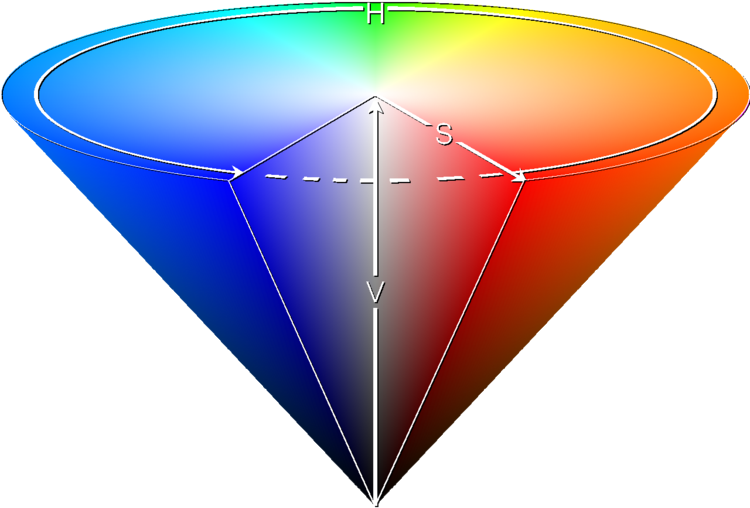
\includegraphics[width=0.45\textwidth,bb=0 0 750 508]{hsv-cone.png}%
   \caption{The HSV color space.}
   \label{fig:hsv-cone}
\end{figure}

\section{Color interpolation}
\index{Color!interpolation}
From studying the RGB cube, we hope you will have understood that there are different routes to follow between two colors, depending whether you are in the RGB or HSV system. Suppose you would make an interpolation between blue and red. In the RGB system you would follow a path diagonally across a face of the cube, from 0/0/255 (blue) via 127/0/127 (purple) to 255/0/0 (red). In the HSV system, you would trace two edges, from 240-1-1 (blue) via 300-1-1 (magenta) to 360-1-1 (red). That is even assuming software would be smart enough to go the shorter route. More likely, red will be recorded as 0-1-1, so hue will be interpolated the other way around, reducing hue from 240\DS\ to 0\DS, via cyan, green, and yellow.

Depending on the design of your color palette, you may want to have it either way. By default, \GMT\ interpolates in RGB space, even when the original color palette is in the HSV system. However, when you add the line \texttt{\#COLOR\_MODEL=+HSV} (with the leading `+' sign) in the header of the color palette file, \GMT\ will not only read the color representation as HSV values, but also interpolate colors in the HSV system. That means that H, S, and V values are interpolated linearly between two colors, instead of their respective R, G, and B values.

The top row in Figure~\ref{fig:GMT_color_interpolate} illustrates two examples: a blue-white-red scale (the \textsf{polar} palette in Appendix~\ref{app:M}) interpolated in RGB and the \textsf{rainbow} palette interpolated in HSV. The bottom row of the Figure demonstrates how things can go terribly wrong when you do the interpolation in the other system.

\begin{figure}[h]
   \centering
   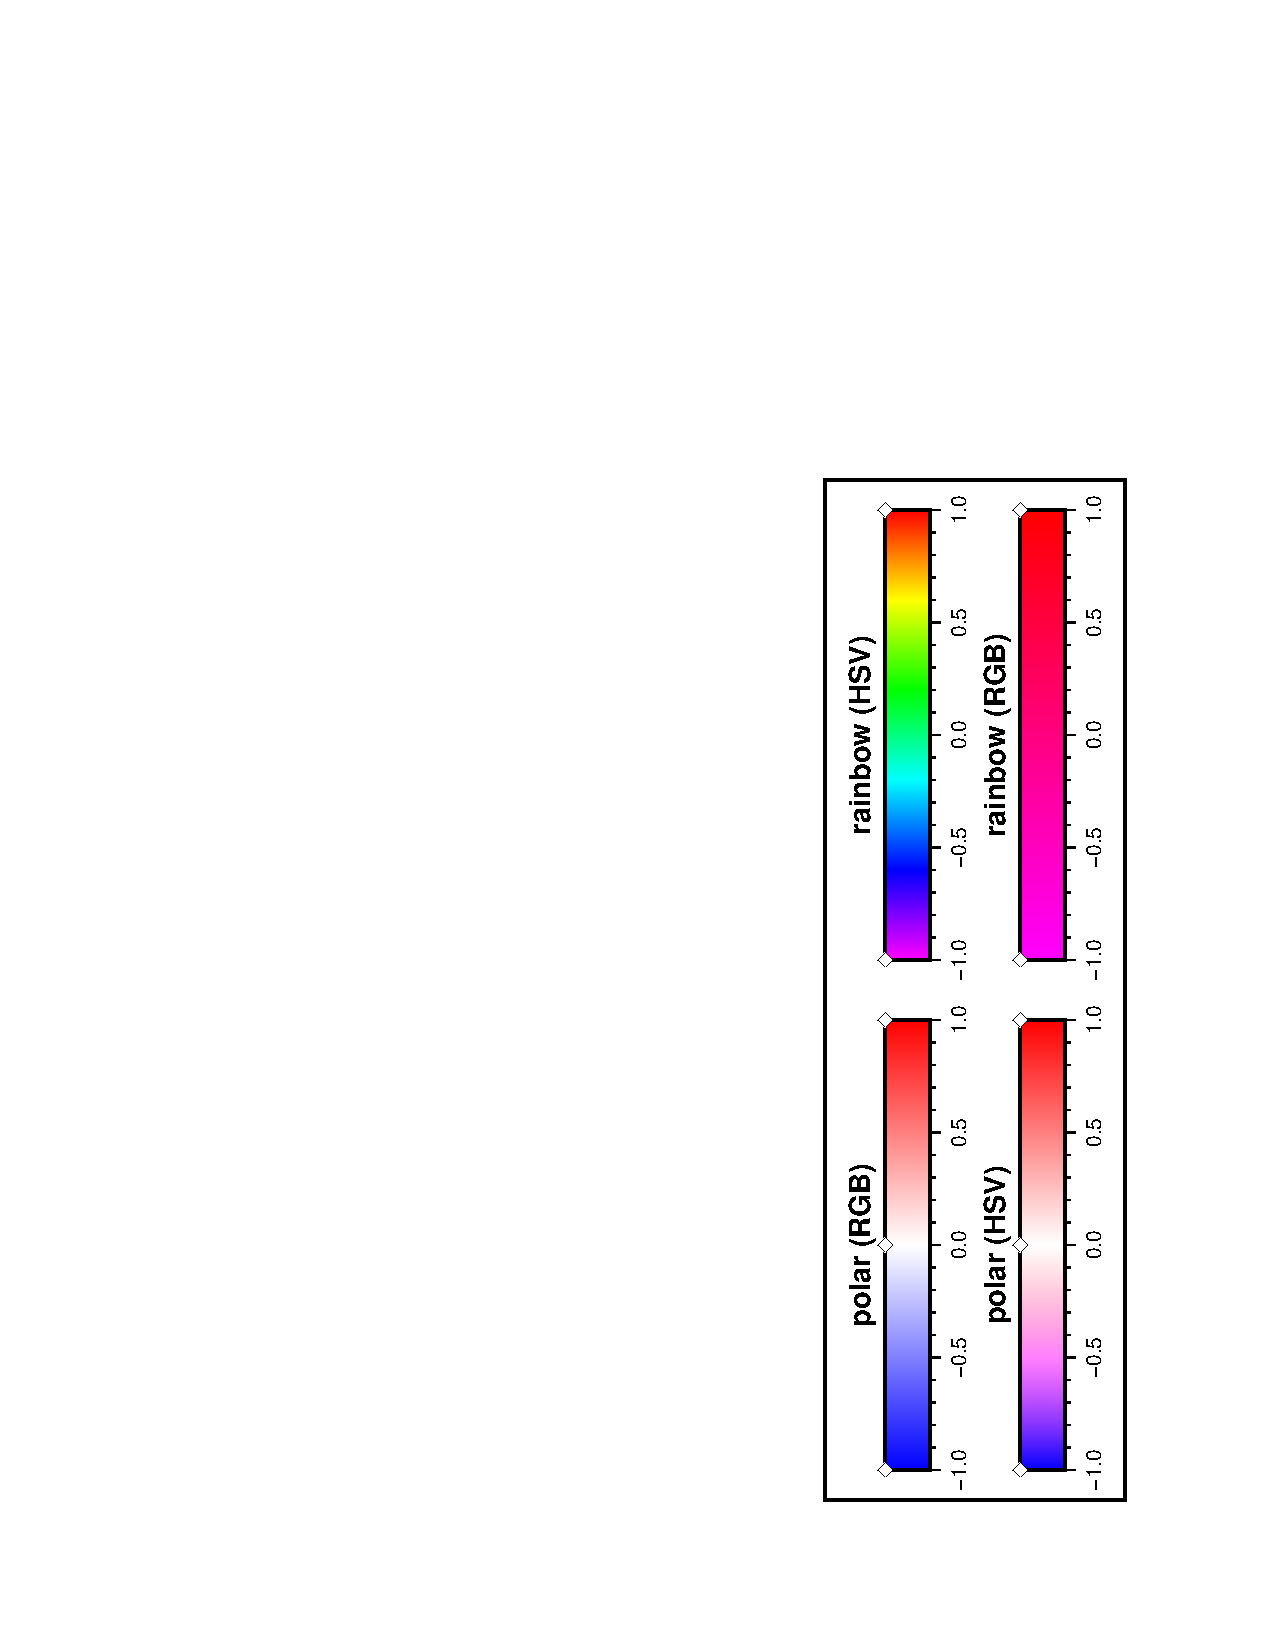
\includegraphics[width=0.80\textwidth]{GMT_color_interpolate}%
   \caption{When interpolating colors, the color system matters. The polar palette on the left needs to be interpolated in RGB, otherwise hue will change between blue (240\DS) and white (0\DS). The rainbow palette should be interpolated in HSV, since only hue should change between magenta (300\DS) and red (0\DS). Diamonds indicate which colors are defined in the palettes; they are fixed, the rest is interpolated.}
   \label{fig:GMT_color_interpolate}
\end{figure}

\section{Artificial illumination}
\index{Illumination, artificial}
\index{Artificial illumination}
\GMT\ uses the HSV system to
achieve artificial illumination of colored images (e.g. \Opt{I}
option in \GMTprog{grdimage}) by changing the saturation \emph{s} and value \emph{v}
coordinates of the color.  When the intensity is zero (flat illumination), the data
are colored according to the CPT file.  If the intensity is
non-zero, the color is either lightened or darkened depending on the illumination.
The color is first converted to HSV (if necessary) and then
darkened by moving ($s$,$v$) toward (\textbf{COLOR\_HSV\_MIN\_S},
\textbf{COLOR\_HSV\_MIN\_V}) if the intensity is negative, or lightened by sliding ($s$,$v$) toward
(\textbf{COLOR\_HSV\_MAX\_S}, \textbf{COLOR\_HSV\_MAX\_V}) if the illumination is positive.
The extremes of the $s$ and $v$ are defined in the \filename{gmt.conf} file and are usually
chosen so the corresponding points are nearly black ($s$ = 1,
$v$ = 0) and white ($s$ = 0, $v$ = 1).
The reason this works is that the HSV system allows movements in
color space which correspond more closely to what we mean by
``tint'' and ``shade''; an instruction like ``add white'' is
easy in HSV and not so obvious in RGB.

\section{Thinking in RGB or HSV}
The RGB system is understandable because it is cartesian, and we all
learned cartesian coordinates in school.  But it doesn't help us
create a tint or shade of a color; we cannot say, ``We want orange,
and a lighter shade of orange, or a less vivid orange''.  With HSV we
can do this, by saying, ``Orange must be between red and yellow, so
its hue is about $h$ = 30\DS; a less vivid orange has a lesser
$s$, a darker orange has a lesser $v$''.  On the other hand,
the HSV system is a peculiar geometric construction, more like a cone (Figure~\ref{fig:hsv-cone}). It is not an
orthogonal coordinate system, and it is not found by a matrix
transformation of RGB; these make it difficult in some cases too.
Note that a move toward black or a move toward white will change both
$s$ and $v$, in the general case of an interior point in the
cube. The HSV system also doesn't behave well for very dark colors,
where the gray point is near black and the two lines we constructed
above are almost parallel.  If you are trying to create nice colors
for drawing chocolates, for example, you may be better off guessing
in RGB coordinates.
\index{Color!HSV system|)}
\index{Color!RGB system|)}

\section{CMYK color system}
\index{Color!CMYK system}
Finally, you can imagine that printers work in a different way: they mix different paints to make a color. The more paint, the darker the color, which is the reverse of adding more light. Also, mixing more colored paints does not give you true black, so that means that you really need four colors to do it right. Open up your color printer and you'll probably find four cartridges: cyan, magenta, yellow (often these are combined into one), and black. They form the CMYK system of colors, each value running from 0 to 1 (or 100\%). In \GMT\ CMYK color coding can be achieved using $c$/$m$/$y$/$k$ quadruplets.

Obviously, there is no unique way to go from the 3-dimensional RGB system to the 4-dimensional CMYK system. So, again, there is a lot of hand waving applied in the transformation. Strikingly, CMYK actually covers a smaller color space than RGB. We will not try to explain you the details behind it, just know that there is a transformation needed to go from the colors on your screen to the colors on your printer. It might explain why what you see is not necessarily what you get. If you are really concerned about how your color plots will show up in your PhD thesis, for example, it might be worth trying to save and print all your color plots using the CMYK system. Letting \GMT\ do the conversion to CMYK may avoid
some nasty surprises when it comes down to printing. To specify the color space of your \PS\ file, set \textbf{PS\_COLOR\_MODEL}
in the \filename{gmt.conf} file to RGB, HSV, or CMYK.
\index{Color|)}
